
La interacción entre los distintos servicios que se desarrollan en este proyecto se realizarán mediante una API. Entre los dos paradígmas más utilizados a la hora de crear APIs se encuentran RPC y REST. Se va a escoger el estandar RPC por responder a los requisistos a los que nos enfrentamos.

\textbf{GRPC}

Según el paper original que describe el paradígma RPC ¨Remote procedure calls (RPC) appear to be a useful paradig m for providing communication across a
network between programs written in a high-level language.¨ \cite{Birrell198439}

RPC permite ejecutar una llamada a un servicio en un servidor remoto mediante formularios predefinidos, obteniendo respuestas con el mismo formato. El estilo del servidor que realiza la llamada, no se tiene en cuenta por diseño.

Google Remote Procedure Call\cite{grpc} - es un subtipo del diseño RPC. gRPC es una arquitectura global de alto rendimiento y de código abierto RPC que garantiza la flexibilidad y la velocidad de la arquitectura de microservicios. Las llamadas a funciones se utilizan gRPC para garantizar la interacción con el cliente en los microservicios creados con varios lenguajes de codificación.

Esta técnica implementa las peticiones de la API en RPC utilizando el estándar HTTP 2.0, pero ni el servidor ni el programador de la API tienen conocimiento de HTTP. Como resultado, la complicación disminuye porque no hay que preocuparse por cómo se traducen los principios de RPC a HTTP.

La llamada a procedimientos remotos de Google pretende acelerar la transferencia de datos entre microservicios. Para permitir la devolución y la llamada remotas, se basa en una estrategia que identifica un servicio, establece las metodologías y especifica las variables pertinentes.

Además, utiliza un IDL -lenguaje de descripción de interfaces- para especificar el paradigma de la API RPC, lo que simplifica la identificación de las funciones remotas. El IDL emplea por defecto Protocol Buffers para definir la interfaz del servicio y el formato de los mensajes de carga útil.

¿Cómo funciona gRPC funciona?

El protocolo HTTP/2, el streaming y los búferes de protocolo o protobufs son utilizados por gRPC APIs para transmitir mensajes. Un estándar de serialización llamado protobuf permite la creación automática de bibliotecas de usuario y la construcción sencilla de microservicios. En los archivos proto, los diseñadores de APIs describen las operaciones y los mensajes que se envían entre servidores y clientes.

El compilador de protoc carga los archivos y crea el software de usuario y servidor para comunicarse con los servicios remotos. En comparación con los formatos XML o JSON, los mensajes codificados con búferes de protocolo son considerablemente más pequeños, lo que hace que el procesamiento sea menos intensivo en CPU.

Además, el uso de HTTP/2, gRPC las API aportan varias mejoras al diseño de RPC. El protocolo añade una capa de formato binario que divide los paquetes en mensajes más pequeños con marco binario, lo que los hace transportables y pequeños. La ejecución de muchas llamadas dentro de un mismo canal es posible gracias al soporte de HTTP/2 para múltiples consultas simultáneas con la arquitectura de comunicación bidireccional.

El protocolo de transporte HTTP/2 admite múltiples flujos simultáneos, pero gRPC Las APIs amplían esta funcionalidad a través de los canales. Cada canal puede albergar varios flujos que se ejecutan simultáneamente a través de muchas conexiones concurrentes. Los canales ofrecen un método sencillo para conectarse al servidor de la API en una dirección y un puerto determinados.

HTTP 1.1 frente a HTTP 2

El enfoque solicitud-respuesta utilizado por las APIs de REST se basa principalmente en HTTP 1.1. Esto significa que el modelo debe procesar cada consulta individualmente si un microservicio recibe muchas consultas de múltiples clientes, lo que arrastra todo el sistema. REST Las APIs pueden desarrollarse sobre HTTP 2, pero como la arquitectura de comunicación sigue siendo petición-respuesta, no pueden aprovechar plenamente las ventajas de HTTP 2, como la compatibilidad bidireccional y la interacción en flujo.

gRPC Las API no se enfrentan a este reto. Se adhiere a un modelo de conexión cliente-respuesta y se basa en HTTP 2. gRPC puede aceptar muchas consultas de varios clientes y procesar esas peticiones al mismo tiempo mediante el flujo de información. Estas circunstancias permiten una comunicación bidireccional con interacción en flujo. Además, gRPC soporta interacciones unarias como las creadas por HTTP 1.1.

gRPC Las APIs pueden gestionar:

\begin{itemize}
    \item Interacciones unarias. Llamada respuesta
    \item Streaming de servidor: una llamada provoca un flujo de mensajes de respuesta del servidor
    \item Streaming de cliente: un flujo de mensajes del cliente provoca una unica respuesta del servidor
    \item Streaming bidireccional: un flujo de mensajes de entrada y salidas independientes
\end{itemize}


\textbf{REST}

REST - Representational State Transfer - es un paradigma cliente-servidor se comunican a través de mensajes codificados en formato JSON o XML o compatibles.

En su disertación original del año 2000, Roy T. Fielding define REST como un "It means that a server will respond with the representation of a resource (today, it will most often be an HTML, XML or JSON document) and that resource will contain hypermedia links that can be followed to make the state of the system change. Any such request will in turn receive the representation of a resource, and so on." \cite{FieldingRoyThomas2000Asat}

Los principios que lo describen son:

\begin{itemize}
    \item Arquitectura cliente-servidor. Hace hincapié en la separación de responsabilidades.
    \item Ausencia de estado. El estado se guarda y mantiene en el cliente y no en el servidor
    \item Habilitación y uso de la caché. Todas las solicitudes deben declarar si son o no cacheables,
    \item Interfaz unifome
    \item Sistema por capas. Tiene relación con la separación de responsabilidades
\end{itemize}


Cada componente que combina el sistema de microservicios puede mostrarse al usuario o al cliente como un recurso cuando la API REST se hace accesible públicamente. Este recurso puede consultarse mediante los comandos HTTP GET, POST, PUT y DELETE .

En una API RESTful, el usuario envía una consulta a una URL - Localizador Uniforme de Recursos, que provoca una respuesta con una carga útil en JSON, XML o cualquier formato de datos compatible. Esta carga útil representa el recurso que desea el usuario. Las peticiones comunes de los clientes incluyen

\begin{itemize}
    \item Un método HTTP que especifica lo que debe procesarse en el recurso
    \item La ruta del recurso
    \item La cabecera que contiene datos sobre la consulta
    \item Una carga útil de mensaje específica del cliente
\end{itemize}


El servidor de la API envía una cabecera de tipo de contenido que identifica el formato de entrega del mensaje empleado en el cuerpo de la respuesta junto con la carga útil de datos que entrega al usuario que realiza la consulta. También se incluye en el cuerpo de la respuesta un código de respuesta que informa al usuario del estado del resultado de la llamada a la API.


\textbf{Compatibilidad con los navegadores}

Dado que la mayor parte de la interacción de la API web se produce en línea, la compatibilidad con el navegador es una consideración clave en el debate entre gRPC vs. REST. La compatibilidad con los navegadores es probablemente una de las principales ventajas de las APIs REST frente a gRPC. Todos los navegadores ofrecen la capacidad completa de la API REST y la compatibilidad con el navegador. Sin embargo, la funcionalidad de gRPC en los navegadores, sin embargo, sigue siendo relativamente restringida. Lamentablemente, las transiciones entre HTTP 1.1 y HTTP 2 necesitan gRPC-web así como una capa proxy. Como resultado, gRPC Las APIs tienden a terminar siendo utilizadas principalmente para sistemas internos o privados, por ejemplo, en aplicaciones API empleadas para la información y funcionalidad del backend de organizaciones específicas.

Con el protocolo HTTP/2 se utilizan flujos multiplexados. Como resultado, numerosos clientes pueden enviar consultas en paralelo sin necesidad de abrir una nueva sesión TCP para cada uno. Además, el servidor puede utilizar el enlace existente para entregar los mensajes a los clientes.

El modelo de transferencia de estado representativo cuenta con un amplio apoyo de los navegadores porque integra HTTP 1.1. HTTP 1.1, que permite REST, utiliza un método de handshaking TCP para cada consulta. REST Por ello, las APIs suelen tener problemas de latencia, ya que el handshake lleva tiempo.

La estructura de datos de la carga útil
Si nos fijamos en la estructura de datos de la carga útil al ver gRPC vs REST, gRPC Las APIs serializan los datos de la carga útil utilizando Protocol Buffers por diseño. Este método es más ligero, ya que hace que los mensajes sean más pequeños y permite una estructura muy comprimida. Los búferes de protocolo están en formato binario; por lo tanto, para el intercambio de datos, serializa y deserializa la información. Protobuf puede traducir automáticamente mensajes muy escritos a los lenguajes de programación del cliente y del servidor.

REST Sin embargo, la mayoría de las veces se utiliza JSON o formularios XML para entregar y recibir información. JSON es el formato más utilizado por su adaptabilidad y capacidad para comunicar datos dinámicos sin atenerse a una estructura precisa, aunque no requiere ninguna. La calidad de lectura humana de JSON, que Protobuf aún no puede igualar, es otra ventaja importante.

JSON no es, sin embargo, tan rápido o ligero cuando se trata de la transferencia de datos. Esto se debe al requisito de que JSON debe ser serializado y traducido a los lenguajes de programación empleados tanto en el extremo del servidor como del cliente cuando se utiliza REST. Se trata de un paso adicional en el proceso de transmisión de datos, que podría perjudicar la eficiencia y aumentar la probabilidad de errores.


\textbf{Generación de código}

Los ingenieros deben emplear herramientas de terceros, como Postman, para la generación de código para las consultas de la API, ya que, a diferencia de gRPCla API REST carece de funciones de generación de código integradas. Por el contrario, , gRPC ofrece funciones de generación de código nativo gracias a su compilador protoc, que admite muchos lenguajes de programación. La generación de código es especialmente ventajosa para los microservicios que combinan numerosos servicios creados en múltiples plataformas y lenguajes. En general, su generación de código integrada facilita la construcción del kit de desarrollo de software (SDK).

REST La API, por otro lado, no proporciona funciones de generación de código nativo. Debe utilizar un programa de terceros para producir la generación de código para las llamadas a la API en varios idiomas. Aunque no es una molestia, es importante tener en cuenta que gRPC no depende de ningún otro servicio para la generación de código.

\textbf{Justificación de uso de gRPC}

Tanto en gRPC vs REST, la mayoría de las herramientas de terceros todavía no proporcionan una funcionalidad integrada para gRPC cumplimiento. En consecuencia, gRPC las API se utilizan sobre todo para crear sistemas o estructuras internas inaccesibles para los usuarios externos. Teniendo en cuenta esta calificación, las siguientes situaciones podrían hacer uso de gRPC APIs:

Conexiones de microservicios
gRPC Las APIs son especialmente útiles para enlazar arquitecturas formadas por microservicios ligeros en los que la eficacia de la entrega de mensajes es crucial debido a su baja latencia y a la rapidez de la comunicación del ancho de banda.

Sistemas multilingües
gRPC destaca en el manejo de las comunicaciones en un contexto políglota gracias a su capacidad de generación de código nativo para una amplia gama de lenguajes de programación.

Transmisión en tiempo real
Si la comunicación en tiempo real es necesaria, su sistema puede transmitir y recibir datos en tiempo real sin tener que esperar a la interacción cliente-respuesta unitaria gracias a la capacidad de gRPC para manejar el streaming bidireccional.

Redes de bajo consumo y bajo ancho de banda
Estas redes pueden beneficiarse del uso de sesiones Protobuf serializadas por parte de gRPC, ya que proporcionan una comunicación ligera, una mayor eficiencia y rapidez. Por ejemplo, una red que se beneficiaría de la gRPC API es el Internet de las cosas.

comparación entre las características de los dos protocolos de comunicación

\begin{figure}[H]
    \centering
    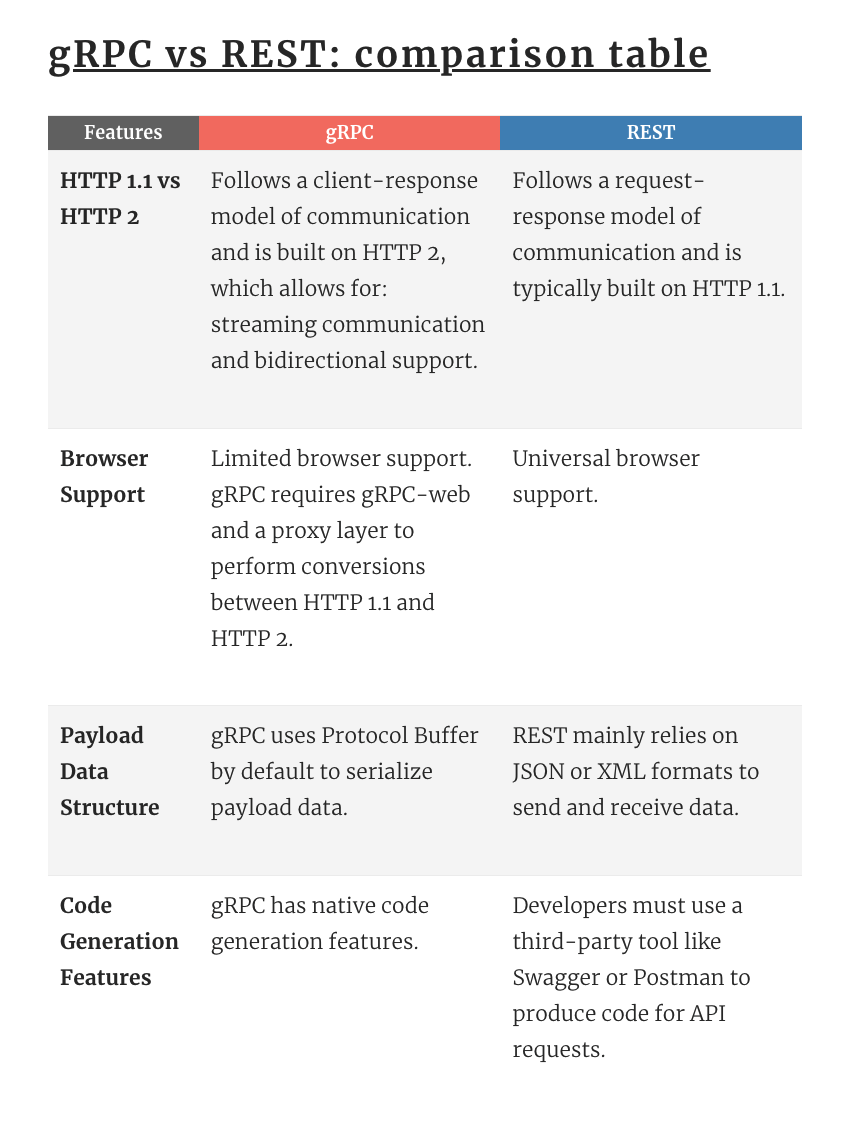
\includegraphics[height=0.3\textheight]{./part/Proyecto_ejecutivo/memoria_constructiva/rpc/img/rpcComparison}
    \caption{gRPC vs REST.\cite{berga_santos_2023}}\label{fig:gRPC vs REST}
\end{figure}

